\section{La Qualité}

	%						%
	%  PREMIERE PARTIE		%
	%						%

\subsection{Développement et tests}

% Première slide %
\begin{frame}
  \frametitle{\color{white} Déroulement du développement et des tests}
  Schéma de Matthieu ici

\end{frame}

% Deuxième slide %
\begin{frame}
  \frametitle{\color{white} Types de tests}
  \begin{itemize}
  \item Tests unitaires
  \item Tests d'intégration
  \item Tests de non-régression
  \item Tests d'acceptation
  \end{itemize}
  
  
\end{frame}


	%						%
	%  SECONDE PARTIE		%
	%						%

\subsection{Stratégie de test}
% Troisième slide %
\begin{frame}
  \frametitle{\color{white} Stratégies des tests}
  \begin{block}{Approche choisie pour les tests}
   Ecriture des tests automatisés puis écriture du code pour faire passer le test
  \end{block}
  \begin{figure}[p]
    \centering
    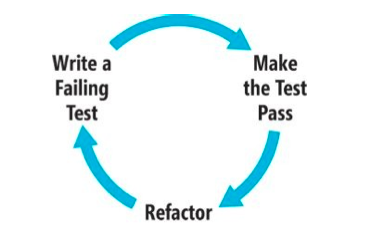
\includegraphics[scale=.25]{tests.png}
    \caption{Développement dirigé par les tests}
  \end{figure}
\end{frame}

% Quatrième slide %
\begin{frame}
  \frametitle{\color{white} Que mettre ici ?}
  TODO : Traiter la gestion du risque de perte d'un membre

\end{frame}


